\section{Energy storage projects in LV application}
\label{ch-literature:sec:energy-storage}

The challenge for DNOs to manage their distribution networks is caused by the DER's and LCT's difficult predictability, their volatile nature, and the weakness of the network into which they are deployed \cite{Woyte2006, Mohd2008a, Koureoumpezis2010, Bravo2015}.
Improved network management methods that are summarised under the term ``smart grid'' have thus become increasingly popular to counteract the negative impact from DERs (e.g. roof-top solar PV) and LCTs (e.g. EVs) \cite{Panteli2015}.
When however deferring the reinforcement or retrofitting of network assets to construct such a smart grid, deployment of BESS can provide a significant contribution to the integration of DERs and LCTs \cite{Grillo2012, Rowe2014a, Li2016, Hosseina2016a}.
As a result, DNOs have begun trialling of BESS across their distribution network to better their understanding and potential contribution \cite{NTVV2016, Lyons2015a, Ferreira2013a}.
%For the scope of reviewing BESS projects and applications in the LV network, both stationary and mobile BESS, i.e. vehicle-to-grid (V2G) enabled EVs, are considered.
To meet statutory and physical restrictions, voltage control and the power flow problem are two identified key challenges \cite{Shi2015}.

%\subsection{Voltage control}

UK distribution networks operate at 230V Phase to Neutral (P2N) or 400V Phase to Phase (P2P) and have a statutory tolerance band of +10\% and -6\%.
Due to the varying load on the network, these voltages can deviate significantly.
Although todays deviation may not exceed the high-voltage or low-voltage thresholds, conduction losses and imperfect network conditions result in a lower overall system efficiency.
Traditionally, OLTC are used to raise and lower voltages across the entire LV distribution network in order to counteract voltage deviations \cite{Sun2009}.
However, such a hierarchical voltage control with OLTCs has its limited applicability, especially in cases where the voltage deviation significantly differs for several branches of a feeding network \cite{Zangs2016}.
Installing a BESS at a strategic location, i.e. closer to the regions where voltage deviation takes place, and controlling the device to best suit the network's requirements is generally applicable and the commercially more viable alternative \cite{Liserre2010}.

As stated by Wade et al. \cite{Wade2009}, allocation of the BESS's limited storage capacity so it can solve the voltage problem most effectively is still a sophisticated challenge.
Nonetheless, by installing a 200kWh unit that is rated at 600kW in a project that was carried out with \textit{EDF Energy}, they showed the potential of BESS in a network to provide targeted voltage support \cite{Wade2010}.
Their results indicate a reduced voltage variation by 2.4\% and a complete elimination of any ``out-of-limit'' voltage events.
A demonstration project in Germany that was titled ``More Microgrids'' used four 180kWh batteries and demonstrated how both voltage stability as well as grid independence could be improved \cite{Overbeeke2010}.
In this project a collection of holiday homes were fitted with a distributed PV system that is capable of generating a peak power of 315kW, and BESS was used to maximise the utility from this generation.
However, due to the relatively small size of the network, due to the different behavioural patterns of holiday home occupants, and due to the different means of connecting customers to the German three-phase network, voltage deviation and phase unbalance issues were less dominant than they would be on a UK distribution feeder.
An equally sized project entitled ``GROWDERS'' also used multiple BESS in the LV network, but instead of focusing at grid independent network operation, they mainly contributed to frequency and thermal constraints as well as voltage stability \cite{GROWDERS2011}.

BESS that are sized between 100kWh to 200kWh (as those in the aforementioned projects \cite{Wade2010, Wade2009, Overbeeke2010, GROWDERS2011}) can easily address network issues, especially even when operating in a grid independent or ``islanded'' mode.
Results from these early field trials show how BESS store the excess renewable power for usage during later times.
But once capacity limits were reached, neither high or low voltage events could be omitted.
An oversized BESS would be less likely to meet its operating limits, but the associated cost makes this oversizing unfeasible.
Their findings therefore indicate that not only the sizing, but also the BESS control method is of significant importance.

%\subsection{Power flow management}

Nonetheless, voltage violations that require strong voltage support have not yet been encountered in any of these projects.
In fact, the majority of low-voltage events on the UK distribution networks, i.e. when voltage levels fall below 216.2V, are caused by anomalous network events or failures of the measurement equipment \cite{UKPowerNetworks2014a}.
Therefore, the complementing task of choosing correct control methods to optimally manage the network's power flow is also important.
This is partly due to measurement equipment in LV substations being more reliable and precise than traditional smart meter readings, but also since it is excessive power flow that causes operational issues which do eventually lead to system overloads and outages \footnote[1]{In fact, according to the UK energy regulator \textit{OFGEM}, on average 45\% of all customers experienced service disruptions in the period 2015-16 \cite{Ofgem2017}. Whilst unanticipated outages due to severe winter weather did lead to \pounds39 million worth of damages, network upgrades to prevent outages and repairs after outages had happened, did however contributed the larger amount of customer interruptions and customer minutes lost \cite{Ofgem2014}.}\cite{Putrus2009, Pillai2010}.
To prevent future power flow from exceeding the system's capacity, BESS has been proposed to function as an instantaneous reserve \cite{Kunisch1986a, Kunisch1986}.
The resulting droop control method uses local voltage and frequency measurements to infer the latest loading and stress on the network to issue corresponding BESS control instructions \cite{Engler2005a}.
Droop control is founded on the assumption that network frequency will drop as demand begins to exceed supply, and that voltages along the distribution feeder drop more significantly when load is increased.
Yet as already stated in Section \ref{ch-literature:sec:topology-of-lv-network}, reversed power flow can raise voltage levels, which makes such droop control methods less reliable and potentially unsuitable for LV network support.
This problem was also encountered by Riffonneau et al. in \cite{Riffonneau2011}, where they control BESS to solve an optimal power flow problem for grid connected PV systems.
Ultimately, they were able to achieve a 13\% reduction of electricity bills by implementing a rule-based dynamic programming optimiser, and they reduced peak power by successfully integrating PV.
However, they do not consider reactive power within their power management method, although it could free additional network resources and yield benefits to the distribution network.
The reason behind excluding it form their study was due to the potential conflicts that may arise with the proposed voltage control method, which heavily relies on voltage measurements.
Using BESS to reallocate PV generation for maximised self-consumption \cite{SaniHassan2017} or to achieve ``peak-shaving'' behaviour \cite{Bennett2015, DePaola2016} has seen continued interest in the field of BESS power flow management.

\begin{figure}\centering
	\subfloat[]{
		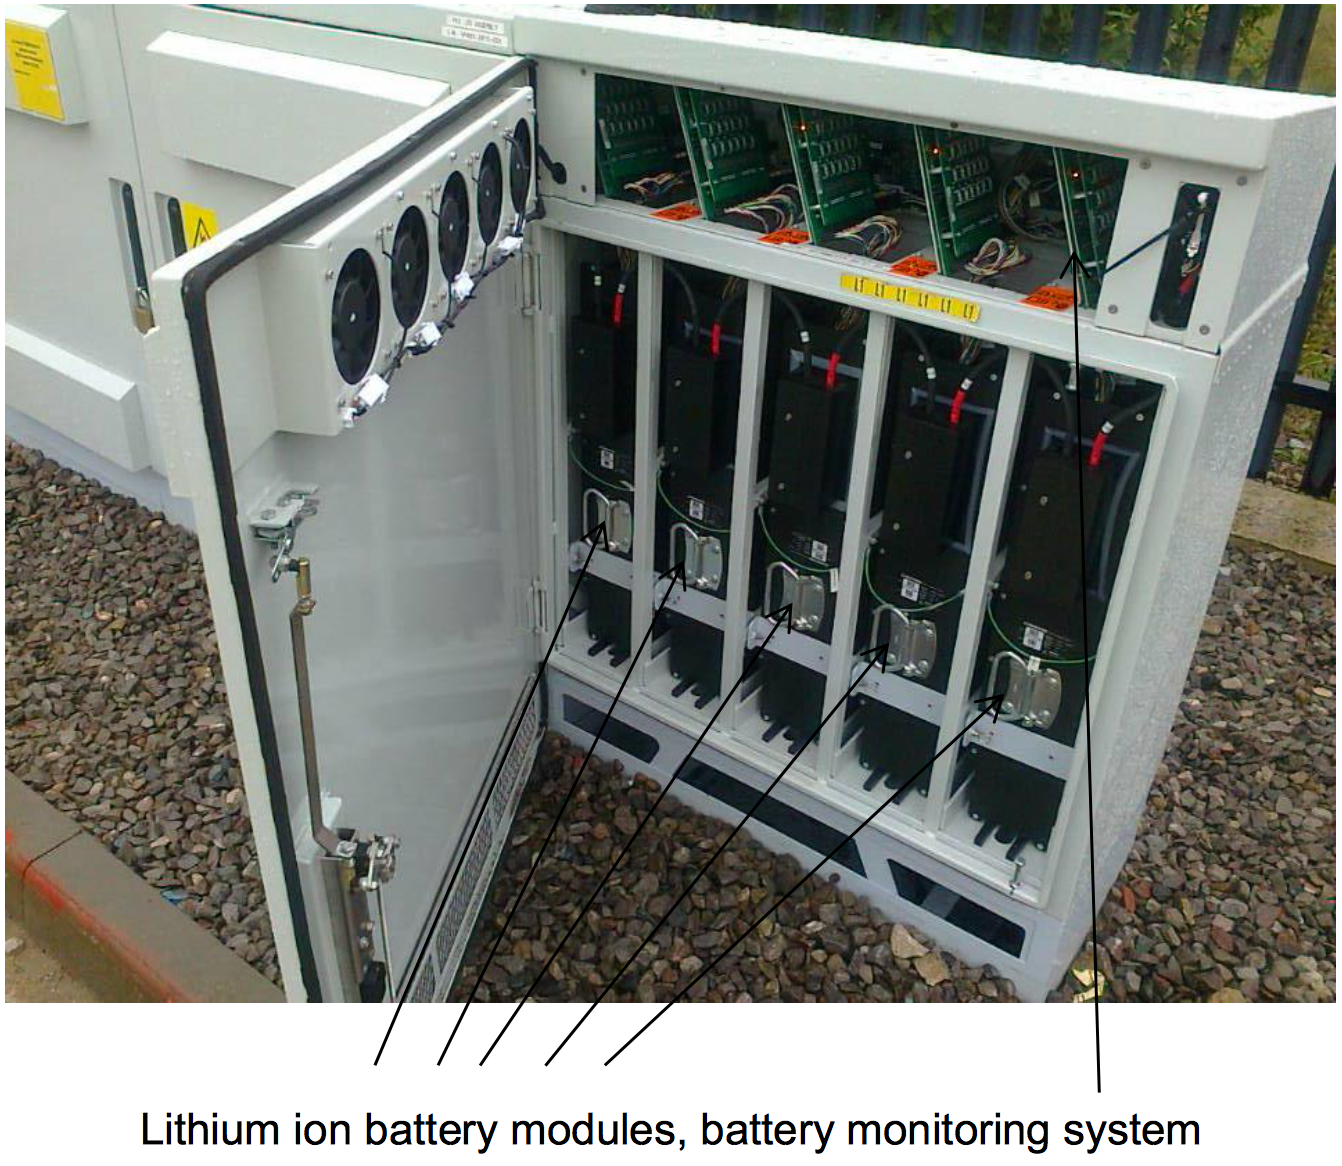
\includegraphics[width=0.415\textwidth]{_literature/fig/esu}
		\label{ch-literature:subfig:esmu-esu}
	}
	\subfloat[]{
		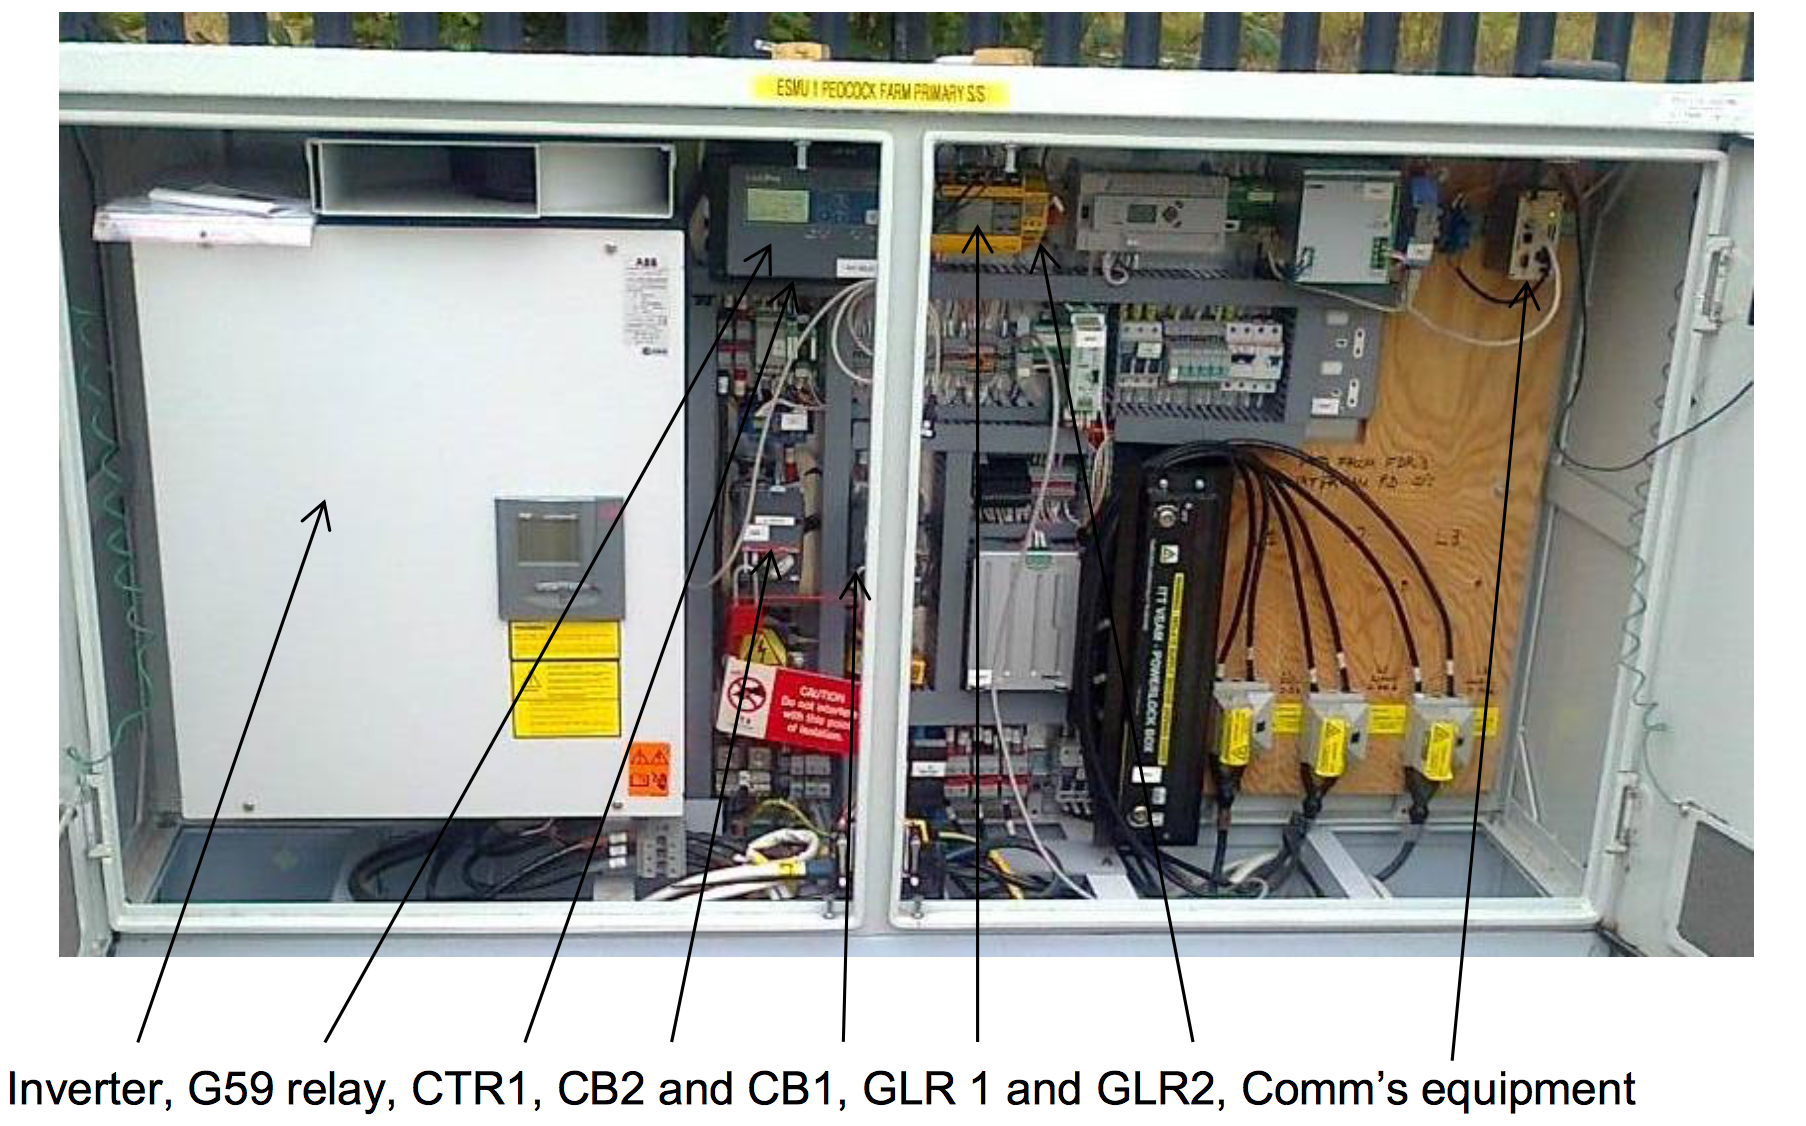
\includegraphics[width=0.585\textwidth]{_literature/fig/peu}
		\label{ch-literature:subfig:esmu-peu}
	}\\
	\subfloat[]{
		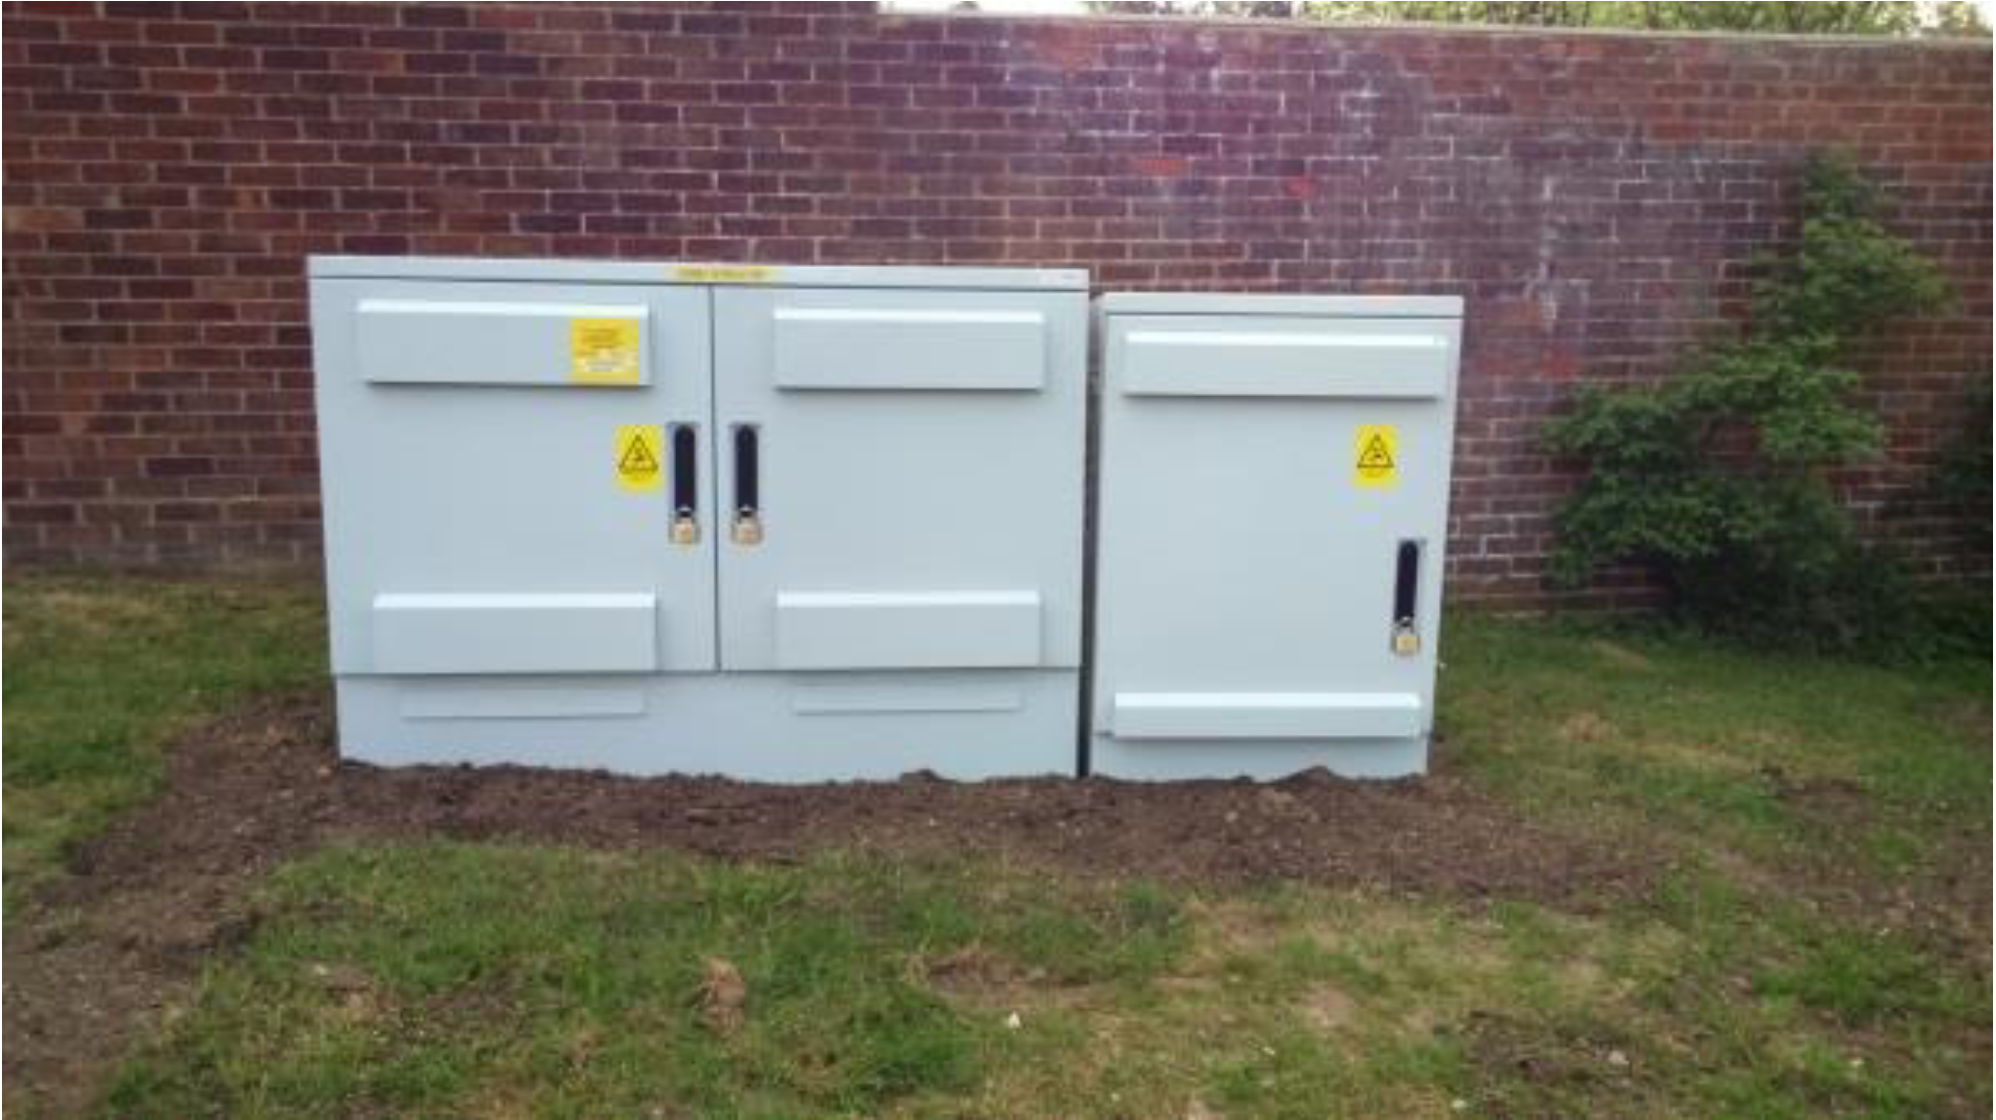
\includegraphics[width=0.7\textwidth]{_literature/fig/esmu-1}
		\label{ch-literature:subfig:esmu-esmu-1}
	}\\
	\subfloat[]{
		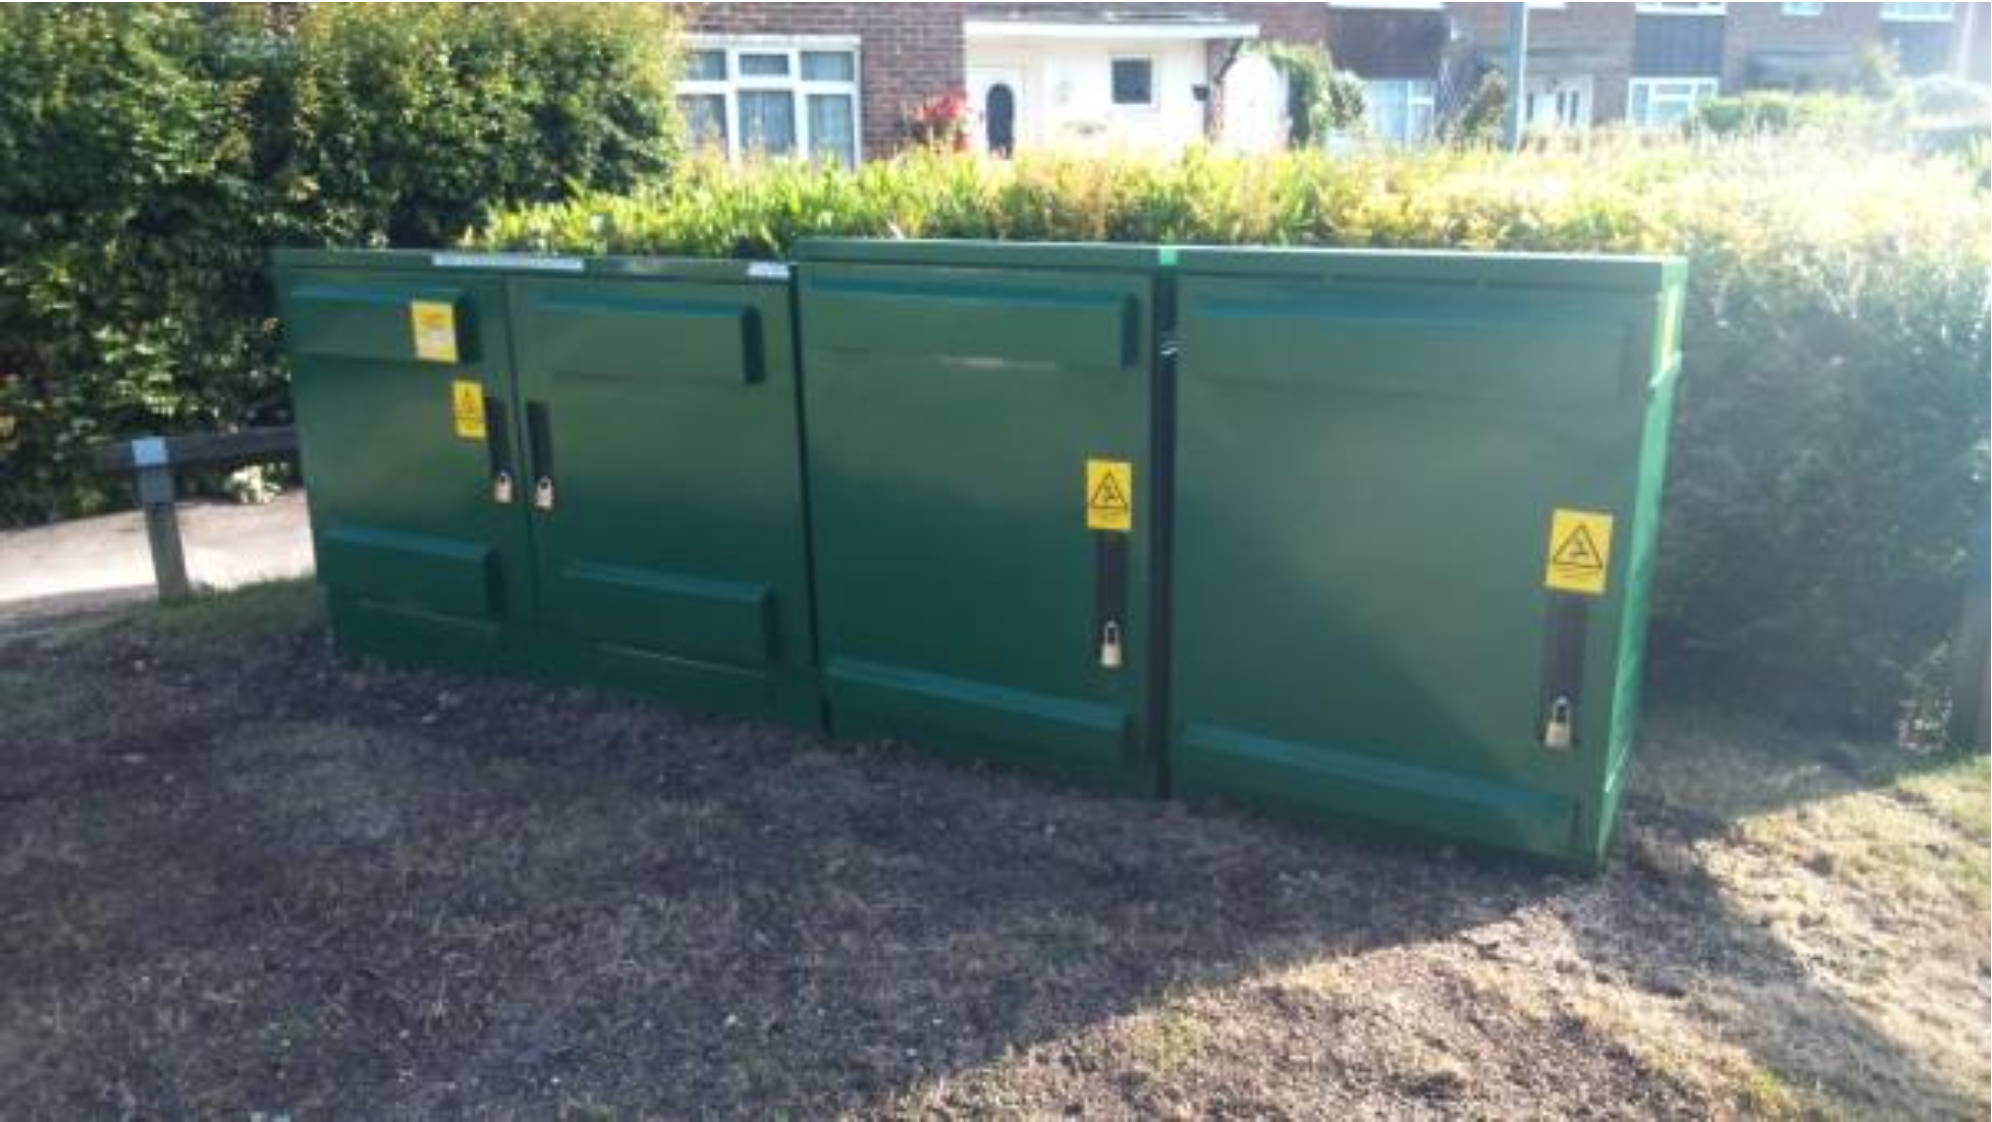
\includegraphics[width=0.7\textwidth]{_literature/fig/esmu-2}
		\label{ch-literature:subfig:esmu-esmu-2}
	}
	\caption{Energy Storage Management Unit overview: (a) 12.5kWh Energy Storage Unit, (b) Power Electronics Unit, (c) deployed 12.5kWh system, (d) deployed 25kWh system - pictures are taken from the NTVV close down report \cite{NTVV9.8a}}
	\label{ch-literature:fig:esmu}
\end{figure}

Aiming to address both voltage and power flow problems, \textit{Scottish and Southern Electricity Networks} (SSEN) became the first UK network operator to trial street-level BESS deployment in the LV network, and they installed 500kWh worth of storage in Bracknell, UK \cite{SSEN2016}.
This capacity was achieved by 25 Energy Storage Management Units (ESMUs), like those pictured in Figure \ref{ch-literature:fig:esmu-esu}.
Each ESMU had cascadable 12.5kWh Energy Storage Units (ESUs), and the ESUs were connected to the distribution network via a three-phase 36kW Power Electronic Unit (PEU) to both manage the batteries and perform filtering operations.
The aim of this so called \textit{New Thames Valley Vision} (NTVV) project was to understand potential benefits, practicalities and costs of installing street-level BESS.
In the beginning, the main problem of finding an optimal deployment location for the ESMUs, to achieve their best possible impact on system voltages had to be addressed.
Yunusov et al. and Rowe et al. in \cite{Yunusov2016, Rowe2014, Rowe2014a} worked in collaboration with \textit{SSEN}, and they assessed different BESS locations in several networks.
They found that a location 4/7 to 2/3 down the feeder yields the best overall impact on voltage levels.
However, their findings also show that this location can vary significantly when not only focusing on voltage support; i.e. proximity to the feeding substation was of greater importance when reducing the system's overloads or distribution losses.
The considered BESS control methods and those implemented in the NTVV project are reviewed in the next section, Section \ref{ch-literature:sec:control-of-energy-storage}.








